% !TEX program = pdflatex
% ============================================================================
% Problem Set 1 - Sección 2: Brecha de ingreso laboral por género
% Deck de diapositivas. Todo número y figura sale de output/, así que el deck
% se mantiene sincronizado con script/05_gender_gap.r: se vuelve a correr ese
% script, se recompila este archivo, y listo. Aquí no hay nada escrito a mano.
%
%   - \input ../../output/tables/gender_gap_stats.tex        (números como macros)
%   - \input ../../output/tables/gender_gap_slide_table.tex  (tabla de resultados)
%   - ../../output/figures/age_income_profile_sex.png        (perfiles por sexo)
%   - ../../output/figures/income_dist_sex.png               (motivación descriptiva)
%
% Compilar desde adentro de presentation/:  pdflatex gender_gap_slides.tex
% Exportar/entregar como gap_equipo_XX.pdf (XX = número de equipo, ver
% \teamnumber abajo).
% ============================================================================
\documentclass[aspectratio=169]{beamer}

\usepackage[utf8]{inputenc}
\usepackage[T1]{fontenc}
\usepackage[spanish,es-noshorthands]{babel}
\usepackage{booktabs}
\usepackage{graphicx}
\usepackage{amsmath}
\usepackage{xcolor}
\usepackage{tikz}
\usetikzlibrary{arrows.meta, positioning, calc}

% uandespurple: acento del deck (títulos de frame, estructura). colmen/colwomen
% coinciden con las dos curvas de la figura de perfiles por sexo
% (05_gender_gap.r), para que las etiquetas de abajo lleven el mismo color que
% el gráfico.
\definecolor{uandespurple}{HTML}{6C0A8A}
\definecolor{colmen}{HTML}{235DA3}
\definecolor{colwomen}{HTML}{AD0D5D}

% alerta/mejora: solo para el waterfall de la descomposición. Deliberadamente
% NO reusamos colmen/colwomen ahí, porque en ese gráfico se leerían como
% "hombres/mujeres" en vez de "la brecha sube / la brecha baja".
\definecolor{alerta}{HTML}{C1440E}
\definecolor{mejora}{HTML}{1B7A43}

% Marca de "corte" (//) sobre el punto medio del segmento #1--#2: rota dos
% barras cortas para que queden siempre perpendiculares a la flecha, sin
% importar su ángulo. La usa el DAG de mediadores.
\newcommand{\cutmark}[2]{%
  \pgfmathanglebetweenpoints{\pgfpointanchor{#1}{center}}{\pgfpointanchor{#2}{center}}%
  \edef\cutang{\pgfmathresult}%
  \coordinate (cm@mid) at ($(#1)!0.5!(#2)$);
  \draw[line width=1.6pt, uandespurple, rotate around={\cutang:(cm@mid)}]
    ($(cm@mid)+(-0.09,-0.19)$) -- ($(cm@mid)+(-0.09,0.19)$);
  \draw[line width=1.6pt, uandespurple, rotate around={\cutang:(cm@mid)}]
    ($(cm@mid)+(0.09,-0.19)$) -- ($(cm@mid)+(0.09,0.19)$);
}

\usetheme{Boadilla}
\setbeamercolor{structure}{fg=uandespurple}
\setbeamercolor{frametitle}{fg=uandespurple}
\setbeamercolor{title}{fg=uandespurple}
\setbeamertemplate{navigation symbols}{}
\setbeamertemplate{caption}[numbered]
\setbeamerfont{frametitle}{size=\large}

% Números clave (brechas, errores estándar, edades pico, IC, ...) como macros.
\newcommand{\GapUncondPct}{21.4}
\newcommand{\GapHKPct}{27.5}
\newcommand{\GapHoursPct}{20.3}
\newcommand{\GapUncondCoef}{-0.240}
\newcommand{\GapHKCoef}{-0.322}
\newcommand{\GapHoursCoef}{-0.227}
\newcommand{\GapHKSE}{0.0132}
\newcommand{\GapHKSEBoot}{0.0131}
\newcommand{\GapRsqUncond}{0.018}
\newcommand{\GapRsqHK}{0.267}
\newcommand{\GapNobs}{14,763}
\newcommand{\GapBootReps}{5,000}
\newcommand{\FWLFull}{-0.32200}
\newcommand{\FWLStageThree}{-0.32200}
\newcommand{\PeakMen}{46.7}
\newcommand{\PeakMenLo}{45.8}
\newcommand{\PeakMenHi}{47.8}
\newcommand{\PeakWomen}{41.9}
\newcommand{\PeakWomenLo}{41.1}
\newcommand{\PeakWomenHi}{42.9}
\newcommand{\PeakDiff}{4.80}
\newcommand{\PeakDiffLo}{3.55}
\newcommand{\PeakDiffHi}{6.09}
\newcommand{\GapAtTwentyFive}{18.9}
\newcommand{\GapAtFortyFive}{30.2}
\newcommand{\GapAtFiftyFive}{37.5}
\newcommand{\PctTertiaryMen}{37.0}
\newcommand{\PctTertiaryWomen}{45.1}
\newcommand{\HoursMen}{50.5}
\newcommand{\HoursWomen}{44.8}
\newcommand{\TenureMen}{66.8}
\newcommand{\TenureWomen}{54.7}


\newcommand{\teamnumber}{XX}

\title[Brecha de género]{La brecha de ingreso laboral por género en Bogotá}
\subtitle{Problem Set 1 \textbullet\ Sección 2}
\author[Perez, Lozano, Suarez]{María José Pérez \and Juan Manuel Lozano \and Samuel Suárez Valle}
\institute[Uniandes]{MECA 4107 --- Big Data y Machine Learning para Economía Aplicada}
\date{Septiembre 2026}

\begin{document}

\begin{frame}[plain]
  \titlepage
\end{frame}

% ---------------------------------------------------------------------------
% Slide 1 (obligatoria): Resultado principal
% ---------------------------------------------------------------------------
\begin{frame}{Resultado principal}
  \begin{block}{Controlar por capital humano \emph{agranda} la brecha, no la reduce}
    \begin{itemize}
      \item \textbf{Brecha incondicional}
        $\bigl(\log w = \beta_1 + \beta_2\,\text{Mujer} + u\bigr)$:
        las mujeres ganan \textbf{\GapUncondPct\,\% menos} al mes
        ($\hat\beta = \GapUncondCoef$).
      \item \textbf{Brecha condicional} (edad, edad$^2$ y educación):
        \textbf{\GapHKPct\,\% menos}
        ($\hat\beta = \GapHKCoef$; EE robusto \GapHKSE, bootstrap \GapHKSEBoot).
        A igual edad y educación la desventaja es \emph{mayor}, porque las
        mujeres de la muestra están más educadas.
      \item \textbf{Perfiles de ciclo de vida:} las mujeres alcanzan su pico de
        ingreso \textbf{\PeakDiff\ años antes} que los hombres
        (IC bootstrap 95\% $[\PeakDiffLo,\ \PeakDiffHi]$), y la brecha se
        ensancha de \GapAtTwentyFive\,\% a los 25 años a
        \GapAtFiftyFive\,\% a los 55.
    \end{itemize}
  \end{block}
  \vfill
  {\footnotesize Muestra: \GapNobs\ ocupados de 18 años o más con ingreso laboral
  positivo, ponderada por \texttt{fex\_c}. Errores estándar robustos a
  heterocedasticidad; bootstrap con \GapBootReps\ repeticiones.}
\end{frame}

% ---------------------------------------------------------------------------
\begin{frame}{Pregunta y decisión metodológica central}
  \textbf{¿Cuánto de la diferencia salarial entre hombres y mujeres persiste al
  comparar trabajadores parecidos, y qué significa ``parecidos''?}
  \vspace{0.6em}
  \begin{itemize}
    
    \item Un \textbf{\emph{bad control}} es una variable que es \emph{consecuencia}
      del género, no una causa. Controlarla no limpia el estimador: le
      quita justamente el canal que queremos medir.\footnote{\scriptsize Cinelli,
        Forney y Pearl (2024), \textit{Sociological Methods \& Research} 53(3):
        1071--1104; Angrist y Pischke (2009), \textit{Mostly Harmless
        Econometrics}, cap.\ 3.}
      \begin{itemize}
        \item Edad y educación son \textbf{predeterminadas} respecto al sexo
          $\Rightarrow$ confusores legítimos.
        \item Ocupación, formalidad y tamaño de empresa son \textbf{resultado} de
          decisiones moldeadas por el género (segregación ocupacional)
          $\Rightarrow$ mecanismos, no confusores.\footnote{\scriptsize Blau y Kahn
            (2017), \textit{Journal of Economic Literature} 55(3): 789--865.}
      \end{itemize}
    \item En general: la brecha condicional fija cuánto de la diferencia
      \emph{no} se explica por características observables --- lo que queda es
      donde vale la pena mirar.
  \end{itemize}
\end{frame}

% ---------------------------------------------------------------------------
\begin{frame}{Datos y decisiones empíricas}
  \begin{itemize}
    \item \textbf{Fuente:} GEIH 2018 (Bogotá), 10 \emph{chunks} scrapeados y combinados.
    \item \textbf{Muestra:} ocupados de 18 años o más con ingreso laboral positivo
      (\GapNobs\ observaciones).
    \item \textbf{Variable dependiente:} $\log$ del ingreso laboral mensual total
      (\texttt{y\_total\_m} $=$ asalariado $+$ independiente).
    \item \textbf{Variable de interés:} \texttt{Mujer} $=1$ si \texttt{sex == 0}
      (codificación del \emph{codebook} de la GEIH).
    \item \textbf{Ponderación:} todas las regresiones usan \texttt{fex\_c}
      (factor de expansión), para que la brecha sea un enunciado sobre los
      trabajadores de Bogotá y no sobre los encuestados.
    \item \textbf{Inferencia:} errores estándar robustos a heterocedasticidad.
      Evaluamos hacer \emph{cluster} por hogar y por ocupación y lo descartamos:
      ninguno es el nivel al que se asigna el sexo (Abadie, Athey, Imbens \&
      Wooldridge, 2023).
  \end{itemize}
\end{frame}

% ---------------------------------------------------------------------------
\begin{frame}{Evidencia descriptiva: por qué la brecha cruda engaña}
  \begin{columns}[T]
    \begin{column}{0.46\textwidth}
      \centering
      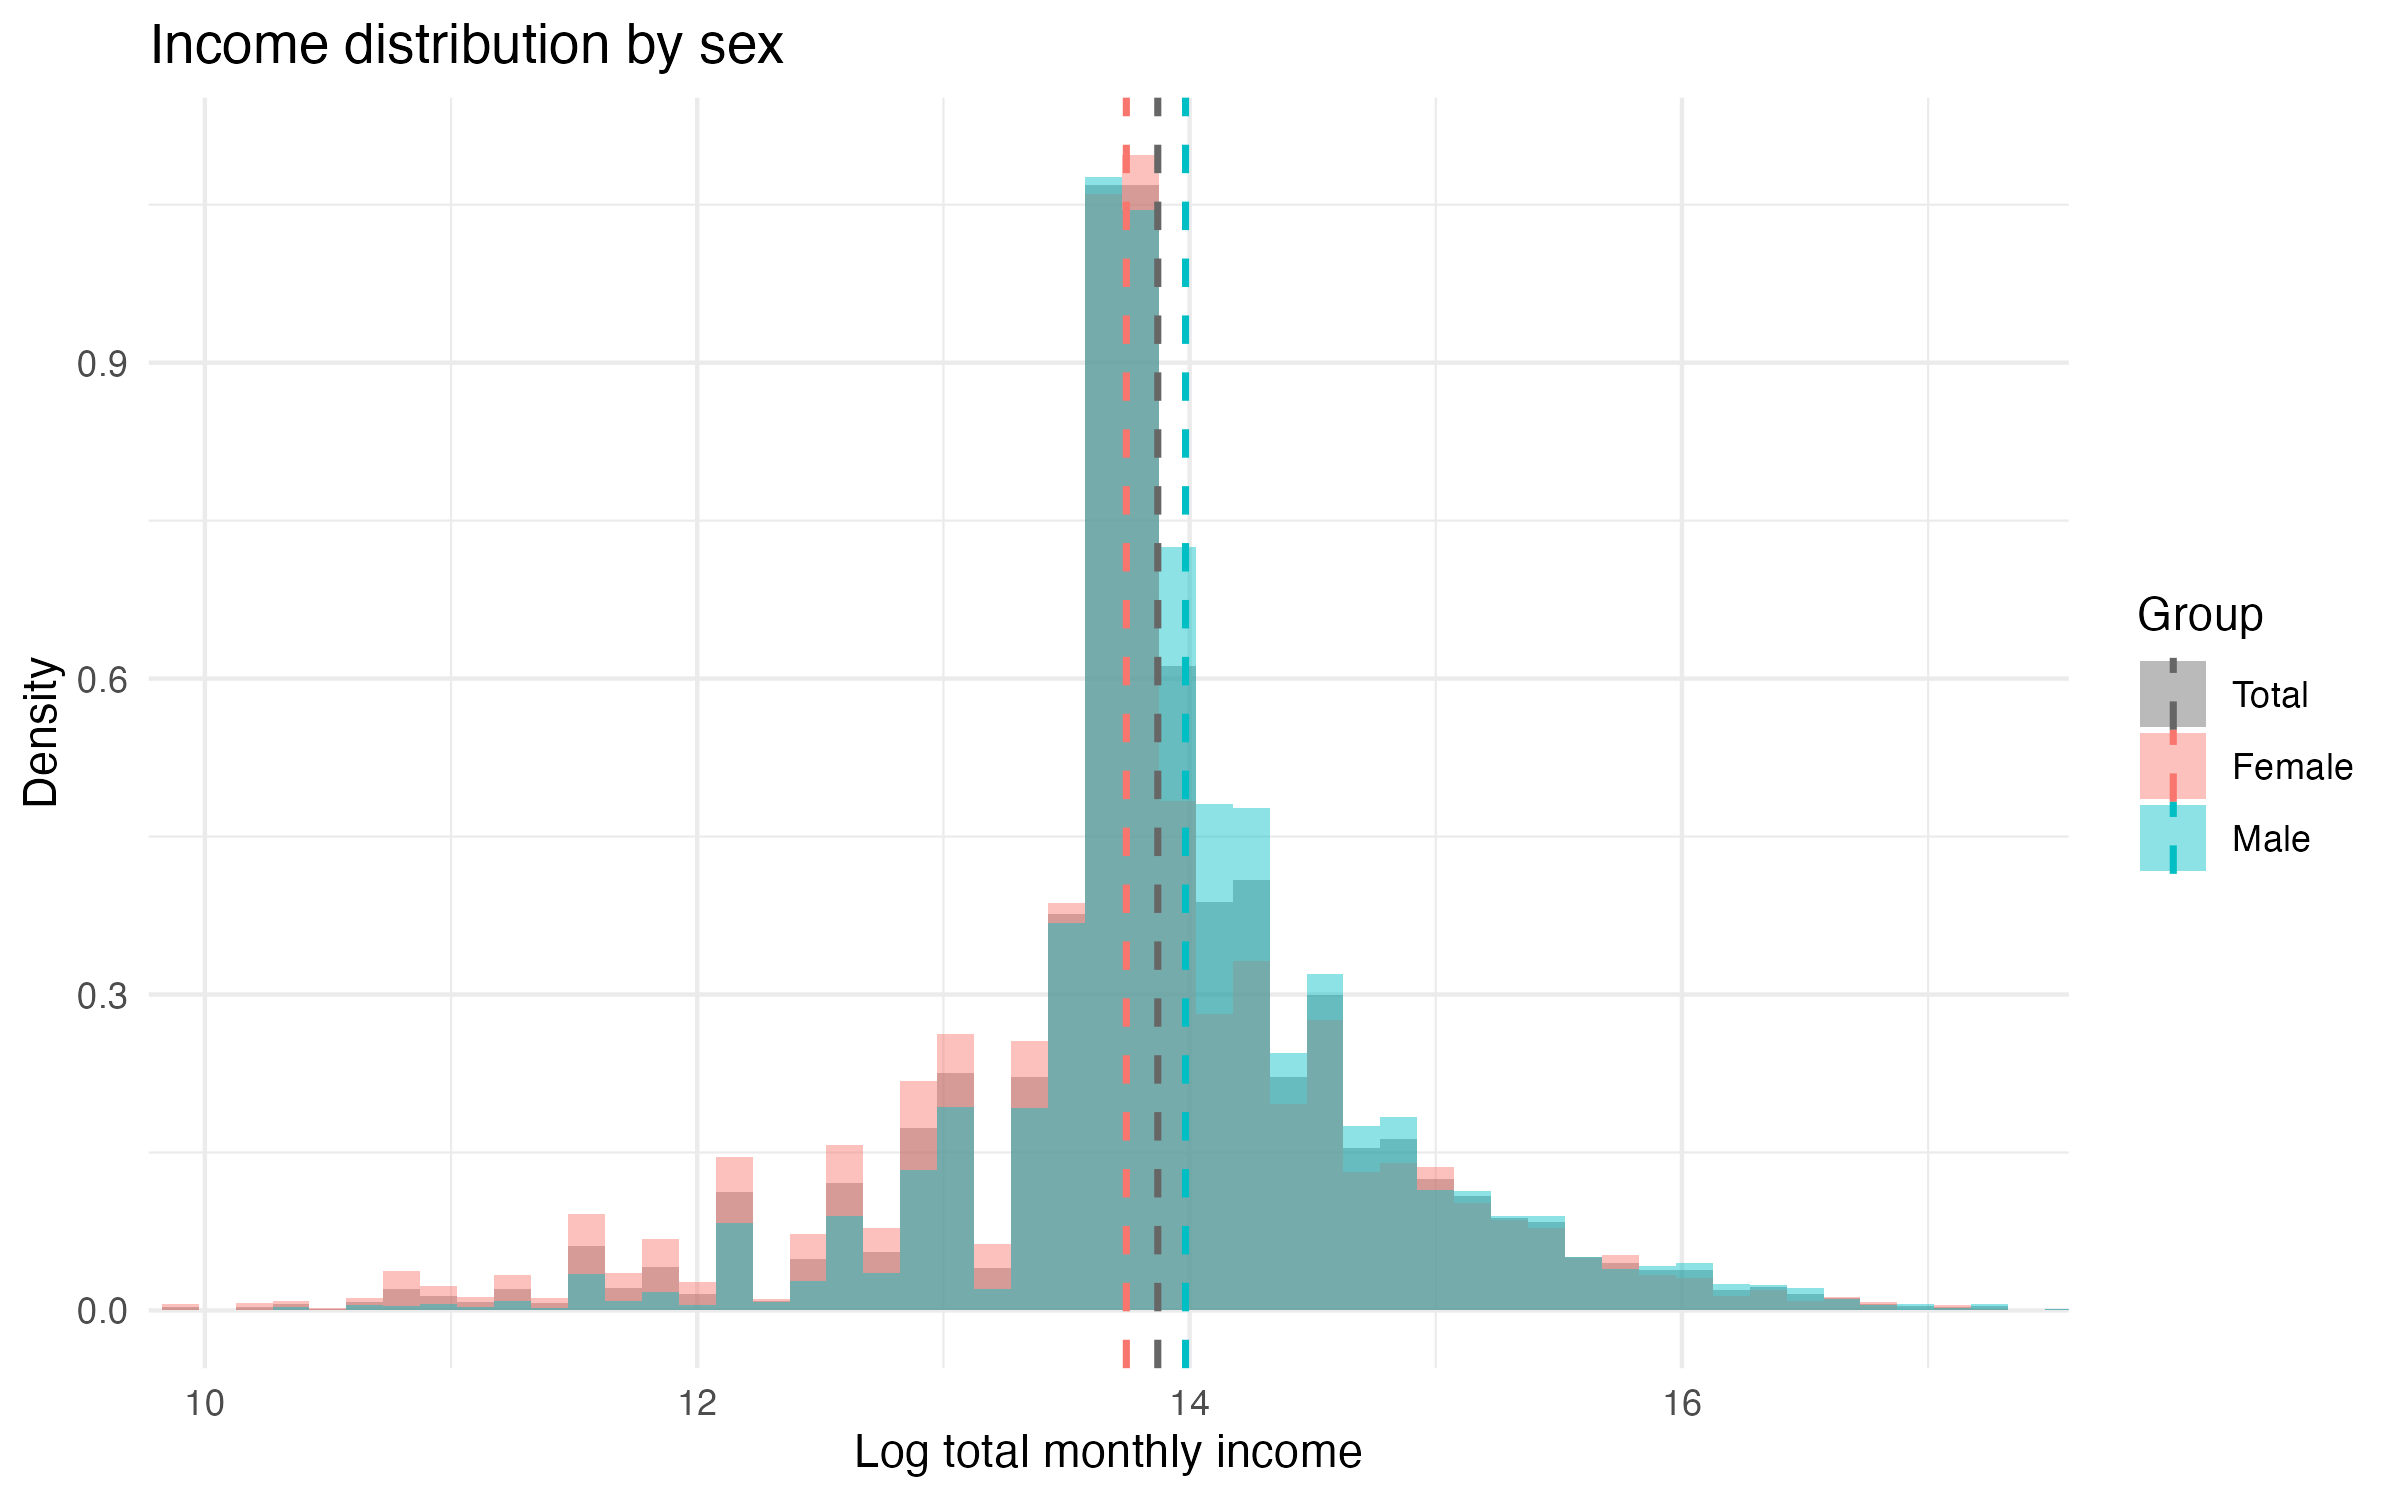
\includegraphics[width=\linewidth]{../../output/figures/income_dist_sex.png}
    \end{column}
    \begin{column}{0.52\textwidth}
      \small
      \begin{tabular}{lcc}
        \toprule
        & \textcolor{colmen}{Hombres} & \textcolor{colwomen}{Mujeres} \\
        \midrule
        Educación terciaria & \PctTertiaryMen\,\% & \PctTertiaryWomen\,\% \\
        Horas por semana    & \HoursMen  & \HoursWomen \\
        Antigüedad (meses)  & \TenureMen & \TenureWomen \\
        \bottomrule
      \end{tabular}
      \vspace{0.8em}
      \begin{itemize}
        \item Las mujeres están \textbf{más} educadas
          (\PctTertiaryWomen\,\% vs.\ \PctTertiaryMen\,\% con terciaria).
        \item Trabajan \textbf{menos horas} pagas y llevan \textbf{menos tiempo}
          en su empleo actual.
        \item Por eso la brecha cruda \emph{subestima} la desventaja: la
          educación la está compensando parcialmente.
      \end{itemize}
    \end{column}
  \end{columns}
\end{frame}

% ---------------------------------------------------------------------------
\begin{frame}{Especificaciones y elección de controles}
  \[
    \log(w_i) = \beta_1 + \beta_2\,\text{Mujer}_i + X_i'\gamma + u_i
  \]
  \vspace{-0.4em}
  \begin{itemize}
    \item \textbf{(1) Incondicional:} $X_i = \varnothing$. Brecha total, con todos
      los canales adentro.
    \item \textbf{(2) Capital humano:} $X_i = \{\text{edad},\ \text{edad}^2,\
      \text{educación}\}$. \emph{Especificación preferida}: son características
      predeterminadas respecto al sexo.
    \item \textbf{(3) $+$ horas trabajadas:} el resultado exigido es el ingreso
      \emph{mensual}, que escala mecánicamente con las horas. Fijarlas acerca la
      estimación a una comparación de \emph{pago por hora} ---
      pero las horas son \textbf{post-tratamiento}: responde otra pregunta, no
      ``mejora'' la (2).
    \item \textbf{No incluimos} ocupación, formalidad ni tamaño de empresa: son
      \emph{bad controls}. Los reportamos como cota inferior de ``a igual
      trabajo'', no como la brecha.
  \end{itemize}
\end{frame}

% ---------------------------------------------------------------------------
\begin{frame}{Qué pregunta responde cada control}
\begin{center}
% Limitado por ALTURA (no por ancho): con la leyenda dentro del lienzo, fijar
% el ancho hacía que el conjunto se saliera por abajo del frame.
\resizebox{!}{6.4cm}{%
\begin{tikzpicture}[
  >=Stealth,
  every node/.style={font=\small},
  endpoint/.style={rectangle, rounded corners=2pt, draw=uandespurple, very thick,
                fill=uandespurple, text=white, font=\bfseries\small,
                minimum width=2.1cm, minimum height=1.0cm, align=center},
  mediator/.style={rectangle, rounded corners=2pt, draw=uandespurple, thick,
                    fill=white, text=black, font=\small,
                    minimum width=2.7cm, minimum height=0.9cm, align=center},
  noconf/.style={rectangle, rounded corners=2pt, draw=gray, thick, dashed,
                  fill=white, text=gray!70!black, font=\small,
                  minimum width=2.1cm, minimum height=0.8cm, align=center},
  direct/.style={-{Stealth[length=3.2mm]}, line width=1.6pt, uandespurple},
  blocked/.style={-{Stealth[length=2.6mm]}, line width=1pt, gray, densely dashed},
  plainarrow/.style={-{Stealth[length=2.6mm]}, line width=1pt, gray!70!black},
  tag/.style={font=\scriptsize\bfseries, uandespurple}
]

\node[endpoint] (sexo) at (0,0) {SEXO};
\node[endpoint] (ingreso) at (11,0) {INGRESO};

\node[mediator] (educ) at (5.5,3.0) {EDUCACIÓN};
\node[mediator] (horas) at (5.5,1.0) {HORAS\\TRABAJADAS};
\node[mediator] (ocup) at (5.5,-2.6) {OCUPACIÓN /\\FORMALIDAD};

\node[noconf] (edad) at (11,-3.6) {EDAD};

% camino directo: lo que queda al bloquear todo lo demás
\draw[direct] (sexo) -- (ingreso);

% caminos mediados: se bloquean al controlar
\draw[blocked] (sexo) -- (educ); \cutmark{sexo}{educ}
\draw[blocked] (educ) -- (ingreso); \cutmark{educ}{ingreso}
\node[tag, above=1pt of educ] {bloqueado en (2)};

\draw[blocked] (sexo) -- (horas); \cutmark{sexo}{horas}
\draw[blocked] (horas) -- (ingreso); \cutmark{horas}{ingreso}
\node[tag, above=1pt of horas] {bloqueado en (3)};

\draw[blocked] (sexo) -- (ocup); \cutmark{sexo}{ocup}
\draw[blocked] (ocup) -- (ingreso); \cutmark{ocup}{ingreso}
\node[tag, below=1pt of ocup, align=center] {no estimado\\en este PS};

% edad: no depende del sexo, solo compone la muestra
\draw[plainarrow] (edad) -- (ingreso);

\node[align=left, font=\scriptsize, text=black, draw=gray!50, fill=white,
      rounded corners=1pt, inner sep=3pt, anchor=north west] at (-1.4,-4.4) {
  {\color{uandespurple}\bfseries --$\to$} efecto directo (persiste en (1)--(3))\\
  {\color{gray} //$\to$} camino bloqueado al controlar (n.\'{u}mero = especificaci\'{o}n)\\
  {\color{gray} - -} EDAD: no depende del sexo, solo compone la muestra
};

\end{tikzpicture}%
}
\end{center}
\footnotesize Cada mediador bloqueado cambia la pregunta que responde el coeficiente de sexo: controlar no elimina un ``sesgo'', redefine la comparación. EDAD entra en (2) pero nunca fue un canal del sexo.
\end{frame}

% ---------------------------------------------------------------------------
\begin{frame}{Resultados: la brecha por especificación}
  \centering
  {\small 
\begin{tabular}[t]{lccccc}
\toprule
Especificación & Mujer & EE robusto & EE bootstrap & Brecha (\%) & $R^2$\\
\midrule
(1) Incondicional & -0.240 & 0.0152 & 0.0151 & -21.4 & 0.018\\
(2) $+$ edad, edad$^2$, educación & -0.322 & 0.0132 & 0.0131 & -27.5 & 0.267\\
(3) $+$ horas trabajadas & -0.227 & 0.0125 & 0.0124 & -20.3 & 0.343\\
\bottomrule
\end{tabular}
}

  \vspace{0.8em}
  \begin{itemize}
    \item De (1) a (2) la brecha \textbf{crece} de \GapUncondPct\,\% a
      \GapHKPct\,\%: a igual edad y educación, la desventaja es mayor.
    \item De (2) a (3) \textbf{cae} a \GapHoursPct\,\%: cerca de un tercio de la
      brecha mensual es diferencia de \emph{horas}, no de tarifa por hora.
    \item Los errores analíticos y bootstrap coinciden en las tres
      especificaciones --- el \emph{pairs bootstrap} es asintóticamente
      equivalente al estimador robusto.
  \end{itemize}
  \vspace{0.3em}
  {\footnotesize Regresiones ponderadas por \texttt{fex\_c}. Bootstrap con
  \GapBootReps\ remuestreos de individuos.}
\end{frame}

% ---------------------------------------------------------------------------
\begin{frame}{La brecha crece al controlar por capital humano}
\begin{center}
\resizebox{!}{6.0cm}{%
\begin{tikzpicture}[
  every node/.style={font=\small},
  total/.style={draw=uandespurple, very thick, fill=uandespurple!18},
  down/.style={draw=alerta, very thick, fill=alerta!75},
  up/.style={draw=mejora, very thick, fill=mejora!75},
  conn/.style={draw=gray, densely dotted, line width=0.6pt},
  vlabel/.style={font=\footnotesize\bfseries},
  clabel/.style={font=\scriptsize, align=center}
]

\def\s{0.15} % cm por punto porcentual

\draw[gray!60, dashed, line width=0.4pt] (-0.6,-10*\s) -- (10.6,-10*\s);
\draw[gray!60, dashed, line width=0.4pt] (-0.6,-20*\s) -- (10.6,-20*\s);
\draw[gray!60, dashed, line width=0.4pt] (-0.6,-30*\s) -- (10.6,-30*\s);
\node[font=\tiny, gray!70!black, anchor=east] at (-0.7,-10*\s) {-10\,\%};
\node[font=\tiny, gray!70!black, anchor=east] at (-0.7,-20*\s) {-20\,\%};
\node[font=\tiny, gray!70!black, anchor=east] at (-0.7,-30*\s) {-30\,\%};
\draw[gray!80, line width=0.6pt] (-0.6,0) -- (10.6,0);
\node[font=\tiny, gray!70!black, anchor=east] at (-0.7,0) {0\,\%};

\draw[total] (0,0) rectangle (1.6,-21.4*\s);
\node[vlabel, uandespurple, anchor=north] at (0.8,-21.4*\s-0.08) {-21,4\,\%};
\node[clabel, anchor=north] at (0.8,-33*\s) {Brecha cruda\\(sin controles)};

\draw[down] (2.1,-21.4*\s) rectangle (3.7,-27.5*\s);
\node[text=white, font=\scriptsize\bfseries] at (2.9,-24.45*\s) {-6,1 pp};
\node[clabel, alerta, anchor=north] at (2.9,-33*\s) {+ edad y\\educación};
\draw[conn] (1.6,-21.4*\s) -- (2.1,-21.4*\s);

\draw[total] (4.2,0) rectangle (5.8,-27.5*\s);
\node[vlabel, uandespurple, anchor=north] at (5.0,-27.5*\s-0.08) {-27,5\,\%};
\node[clabel, anchor=north] at (5.0,-33*\s) {Brecha ajustada\\(capital humano)};
\draw[conn] (3.7,-27.5*\s) -- (4.2,-27.5*\s);

\draw[up] (6.3,-27.5*\s) rectangle (7.9,-20.3*\s);
\node[text=white, font=\scriptsize\bfseries] at (7.1,-23.9*\s) {+7,2 pp};
\node[clabel, mejora, anchor=north] at (7.1,-33*\s) {+ horas\\trabajadas};
\draw[conn] (5.8,-27.5*\s) -- (6.3,-27.5*\s);

\draw[total] (8.4,0) rectangle (10.0,-20.3*\s);
\node[vlabel, uandespurple, anchor=north] at (9.2,-20.3*\s-0.08) {-20,3\,\%};
\node[clabel, anchor=north] at (9.2,-33*\s) {Brecha\\por hora};
\draw[conn] (7.9,-20.3*\s) -- (8.4,-20.3*\s);

\end{tikzpicture}%
}
\end{center}
\footnotesize Al fijar edad y educación la brecha \textbf{se amplía} (rojo): las mujeres de la muestra tienen más educación terciaria (\PctTertiaryWomen\,\% vs.\ \PctTertiaryMen\,\%), así que la brecha subestimaba la desventaja. Al fijar además horas trabajadas, se reduce (verde).
\end{frame}

% ---------------------------------------------------------------------------
\begin{frame}{Frisch--Waugh--Lovell: el mismo coeficiente, por construcción}
  \begin{columns}[T]
    \begin{column}{0.46\textwidth}
      \textbf{El procedimiento}
      \begin{enumerate}
        \item Regresar $\log w$ contra los controles $\rightarrow$ residuos.
        \item Regresar Mujer contra los mismos controles $\rightarrow$ residuos.
        \item Regresar unos residuos contra los otros.
      \end{enumerate}
      \vspace{0.8em}
      \centering
      \begin{tabular}{lc}
        \toprule
        & $\hat\beta_{\text{Mujer}}$ \\
        \midrule
        Regresión completa & \FWLFull \\
        FWL (etapa 3)      & \FWLStageThree \\
        \bottomrule
      \end{tabular}
    \end{column}
    \begin{column}{0.52\textwidth}
      \textbf{Por qué coinciden}
      \vspace{0.4em}

      Las etapas 1 y 2 le quitan a cada variable todo lo que la edad y la
      educación pueden explicar. Lo que queda de \emph{Mujer} es la variación
      \textbf{ortogonal a los controles} --- exactamente la variación que la
      regresión completa usa para identificar el coeficiente.
      \vspace{0.6em}

      No son dos estimadores distintos: es \textbf{el mismo estimador} calculado
      de dos formas. La diferencia entre ambos es de orden $10^{-14}$, es decir
      error de redondeo de punto flotante.
    \end{column}
  \end{columns}
  \vfill
  {\footnotesize El error estándar de la etapa 3 sale $0{,}02\%$ menor porque
  \texttt{feols} no sabe que las etapas 1 y 2 ya consumieron grados de libertad
  ($n-2$ en vez de $n-k$). Reescalándolo por $\sqrt{(n-2)/(n-k)}$ coincide
  exactamente con el de la regresión completa.}
\end{frame}

% ---------------------------------------------------------------------------
\begin{frame}{Perfiles edad--ingreso por sexo}
  \centering
  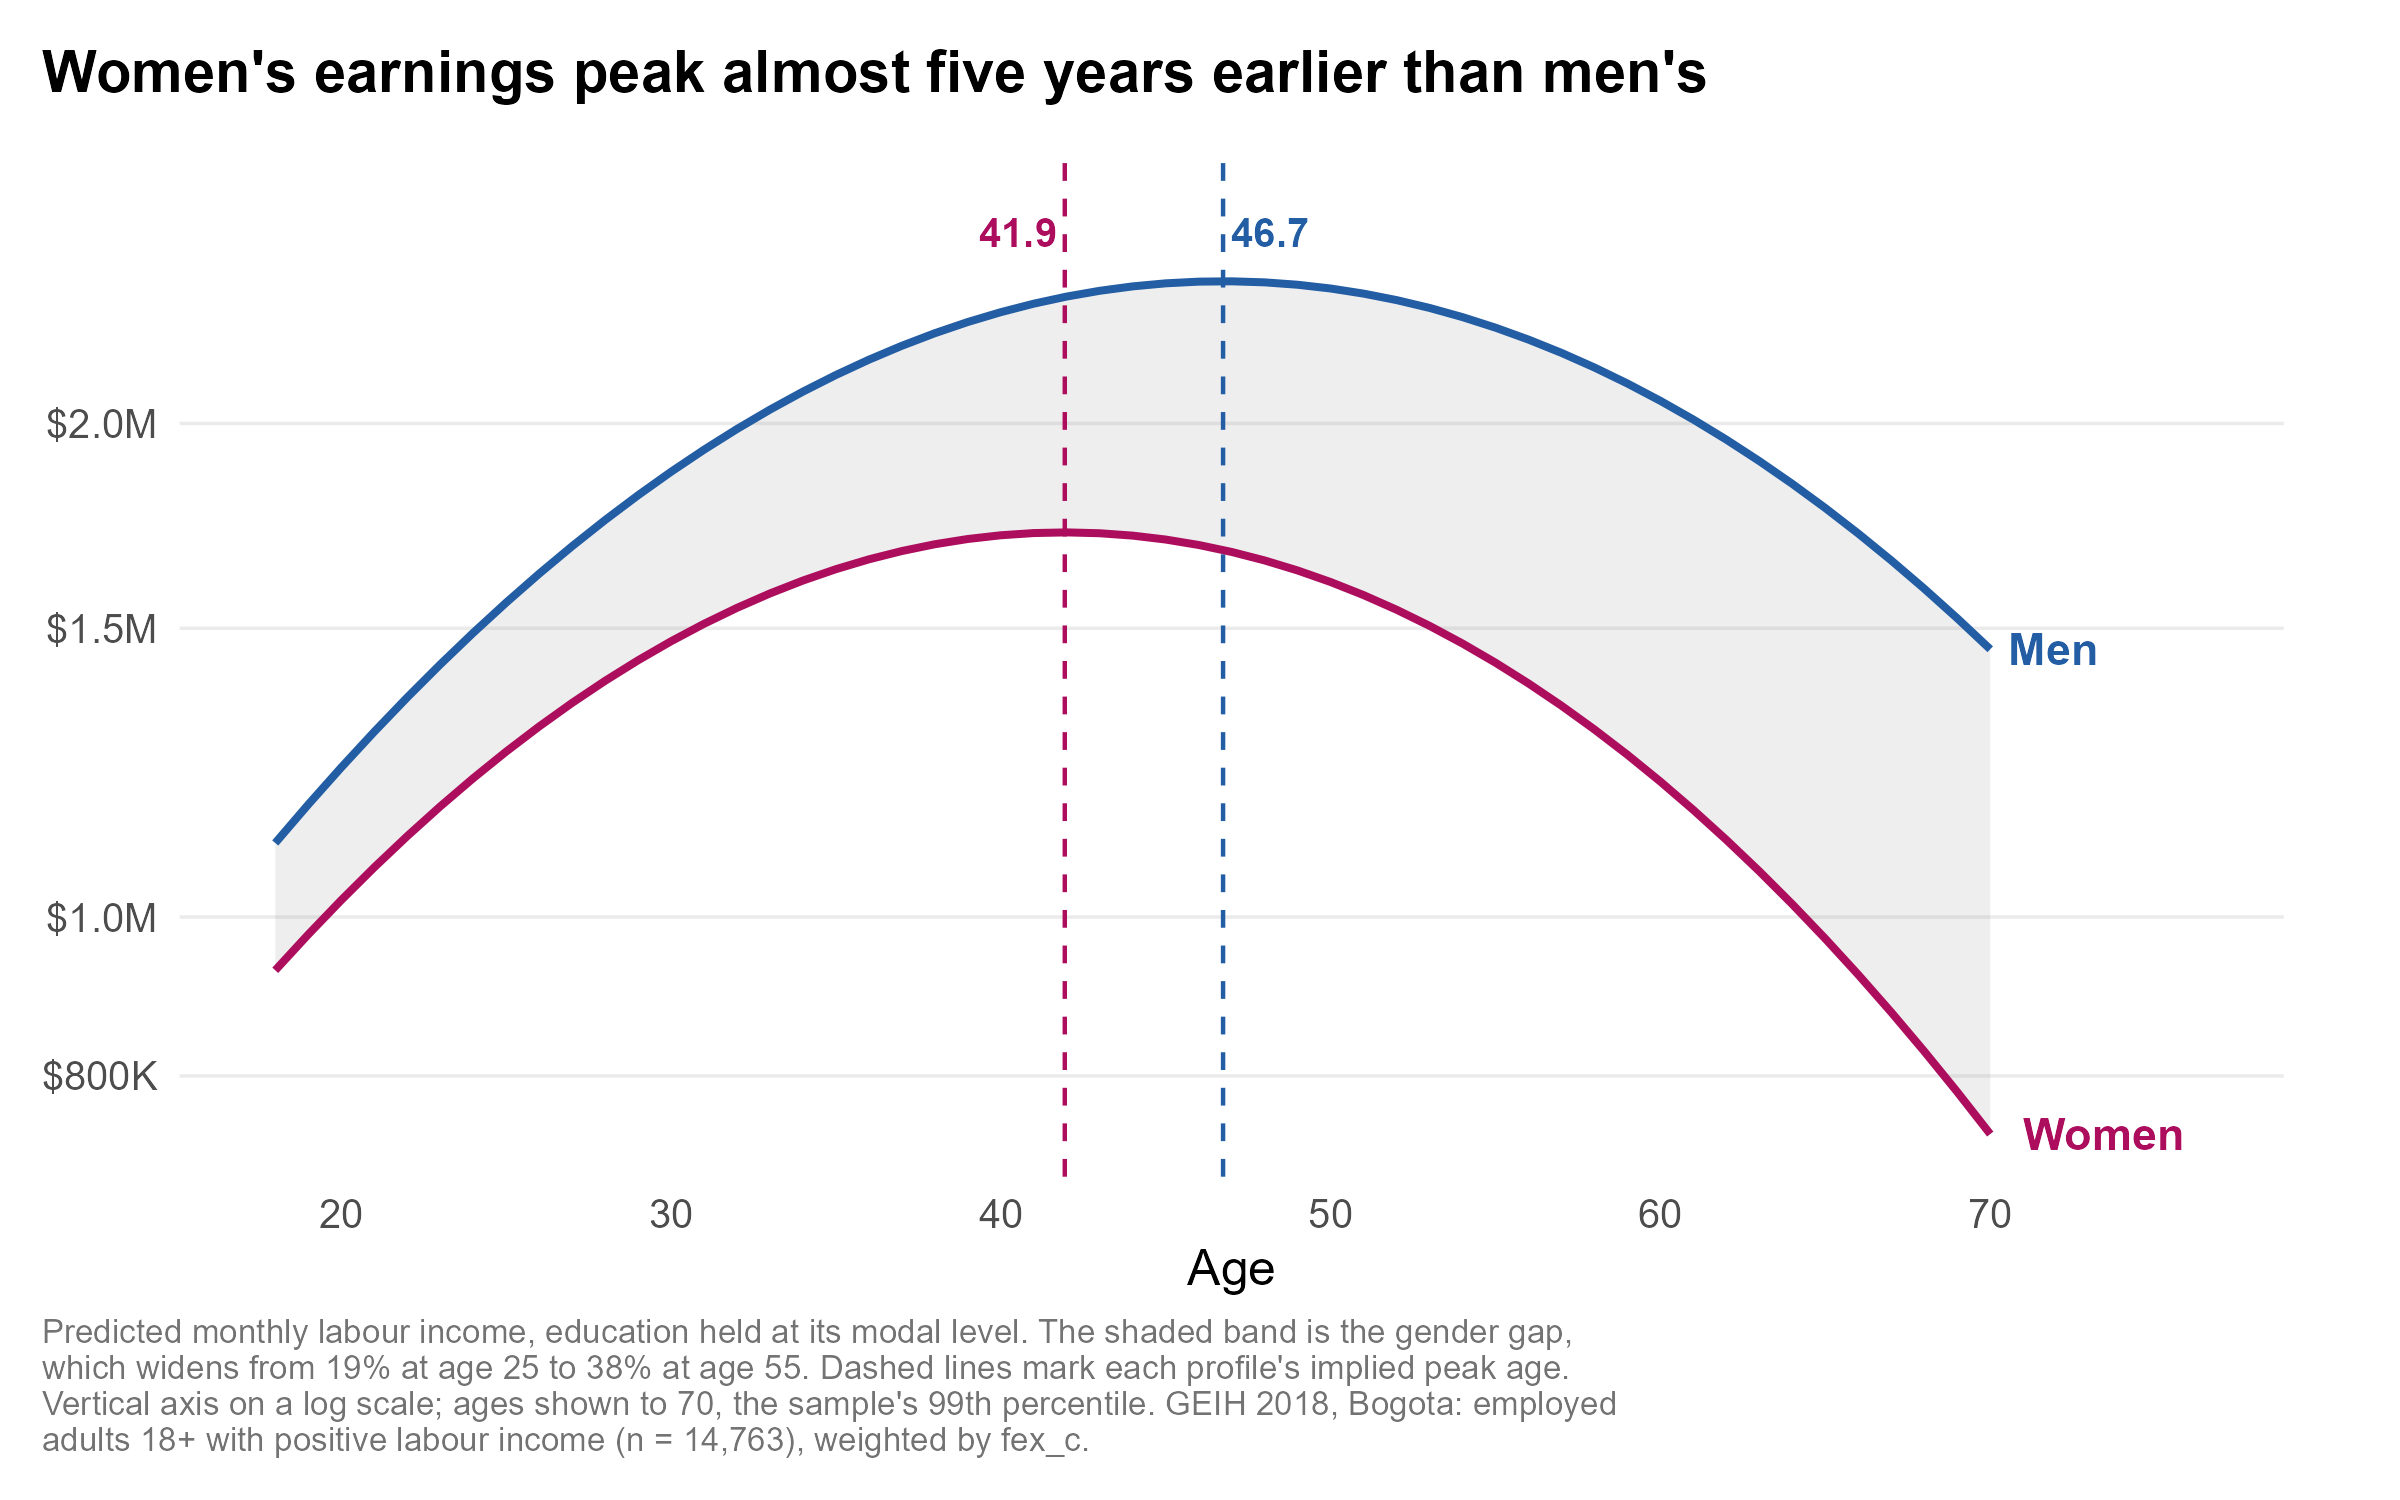
\includegraphics[height=0.76\textheight]{../../output/figures/age_income_profile_sex.png}

  {\footnotesize Especificación con interacciones
  $\text{Mujer}\times\text{edad}$ y $\text{Mujer}\times\text{edad}^2$: sin ellas
  ambos sexos compartirían la misma curvatura y la misma edad pico, y la
  comparación sería vacua. La banda sombreada es la brecha a cada edad.}
\end{frame}

% ---------------------------------------------------------------------------
\begin{frame}{Edad pico por sexo: la brecha se ensancha con la edad}
  \begin{columns}[T]
    \begin{column}{0.44\textwidth}
      \centering
      \begin{tabular}{lcc}
        \toprule
        & Edad pico & IC 95\% \\
        \midrule
        \textcolor{colmen}{Hombres} & \PeakMen &
          $[\PeakMenLo,\ \PeakMenHi]$ \\
        \textcolor{colwomen}{Mujeres} & \PeakWomen &
          $[\PeakWomenLo,\ \PeakWomenHi]$ \\
        \midrule
        \textbf{Diferencia} & \textbf{\PeakDiff} &
          $\mathbf{[\PeakDiffLo,\ \PeakDiffHi]}$ \\
        \bottomrule
      \end{tabular}
      \vspace{0.8em}

      {\footnotesize Brecha implícita por edad:\\
      25 años: \GapAtTwentyFive\,\% \quad
      45 años: \GapAtFortyFive\,\% \quad
      55 años: \GapAtFiftyFive\,\%}
    \end{column}
    \begin{column}{0.54\textwidth}
      \begin{itemize}
        \item El IC de la diferencia \textbf{no incluye el cero}: los hombres
          alcanzan su pico significativamente más tarde.
        \item \textbf{Lección metodológica:} los coeficientes de interacción
          \emph{individualmente} no son significativos ($p = 0{,}91$ y
          $p = 0{,}15$), pero su combinación no lineal sí lo es. La significancia
          de una cantidad derivada no se lee de los $t$ de la tabla --- hay que
          testearla directamente, y para eso sirve el bootstrap.
        \item \textbf{Ojo:} con interacciones, el coeficiente de \emph{Mujer} ya
          no es ``la brecha'': mide la brecha en $\text{edad}=0$, una
          extrapolación fuera de la muestra.
      \end{itemize}
    \end{column}
  \end{columns}
\end{frame}

% ---------------------------------------------------------------------------
\begin{frame}{Conclusiones}
  \begin{itemize}
    \item La brecha de género en Bogotá es de \textbf{\GapUncondPct\,\%} sin
      condicionar y \textbf{\GapHKPct\,\%} comparando trabajadores de igual edad
      y educación: controlar por capital humano la \textbf{agranda}, porque las
      mujeres de la muestra están más educadas.
    \item Cerca de un tercio de la brecha \emph{mensual} corresponde a
      diferencias en \textbf{horas trabajadas}, no en pago por hora --- pero
      controlarlas responde una pregunta distinta, no una mejor.
    \item La desventaja \textbf{se acumula a lo largo del ciclo de vida}: las
      mujeres llegan a su pico \PeakDiff\ años antes y la brecha pasa de
      \GapAtTwentyFive\,\% a los 25 a \GapAtFiftyFive\,\% a los 55.
    \item Para la autoridad tributaria: el género predice desviaciones
      sistemáticas del ingreso esperado, pero es un marcador de
      \textbf{desigualdad estructural}, no de sub-reporte --- usarlo como señal
      de fiscalización sería confundir una cosa con la otra.
  \end{itemize}
\end{frame}

\end{document}
